
% =========================================================
% LinkedIn Carousel (Portrait 4:5) — Double Machine Learning
% =========================================================

\documentclass{beamer}

% ----------------------------
% Page: portrait 4:5  (matches 1080 × 1350 px)
% ----------------------------
\setlength{\paperwidth}{14.4cm}
\setlength{\paperheight}{18.0cm}
\setlength{\pdfpagewidth}{\paperwidth}
\setlength{\pdfpageheight}{\paperheight}

% ----------------------------
% Packages
% ----------------------------
\usepackage[T1]{fontenc}
\usepackage{lmodern}
\usepackage{amsmath,amssymb}
\usepackage{booktabs}
\usepackage{graphicx}
\usepackage{tikz}
\usetikzlibrary{arrows.meta,positioning,shapes.geometric,calc}
\usepackage{pgfplots}
\pgfplotsset{compat=1.18}

% PDF outline & metadata
\usepackage{bookmark}
\usepackage{hyperref}
\hypersetup{
  pdftitle    = {Double Machine Learning — Orthogonalization},
  pdfauthor   = {Muiz Olasupo},
  pdfsubject  = {Causal Inference in Economics},
  pdfkeywords = {Double ML, Orthogonalization, Causal Inference},
  bookmarksnumbered = true,
  bookmarksopen     = true,
  bookmarksdepth    = 3,
  pdfstartview      = Fit,
  colorlinks        = false,
}

% ----------------------------
% Colors
% ----------------------------
\definecolor{ink}{RGB}{12,14,18}
\definecolor{muted}{RGB}{100,106,115}
\definecolor{soft}{RGB}{245,247,250}
\definecolor{linegray}{RGB}{210,218,230}
\definecolor{accent}{RGB}{27,100,209}
\definecolor{accentorange}{RGB}{225,108,32}
\definecolor{accentgreen}{RGB}{33,158,115}
\definecolor{accentpurple}{RGB}{120,72,221}

% ----------------------------
% Theme — minimal, portrait-friendly
% ----------------------------
\usetheme{default}

\setbeamersize{text margin left=12mm, text margin right=12mm}

\setbeamercolor{normal text}{fg=ink, bg=white}
\setbeamercolor{frametitle}{fg=ink, bg=white}
\setbeamercolor{structure}{fg=accent}
\setbeamercolor{block title}{fg=ink, bg=soft}
\setbeamercolor{block body}{fg=ink, bg=soft}

\setbeamerfont{frametitle}{size=\Large, series=\bfseries}

\setbeamertemplate{navigation symbols}{}
\setbeamertemplate{headline}{}

% Frame title with subtle separator
\setbeamertemplate{frametitle}{%
  \vspace{8pt}%
  {\usebeamerfont{frametitle}\usebeamercolor[fg]{frametitle}%
   \insertframetitle}%
  \vspace{3pt}%
  {\color{linegray}\rule{\linewidth}{0.4pt}}%
  \vspace{4pt}%
}

% Bullets
\setbeamertemplate{itemize item}{%
  \color{accent}\raisebox{0.15em}{\scriptsize$\blacksquare$}}
\setbeamertemplate{itemize subitem}{%
  \color{accent}\raisebox{0.2em}{\tiny$\blacktriangleright$}}

% Footer — page counter only
\setbeamertemplate{footline}{%
  \begin{beamercolorbox}[wd=\paperwidth,ht=3ex,dp=1.5ex,
    leftskip=12mm,rightskip=12mm]{normal text}%
    \color{muted}\small\hfill
    \insertframenumber\,/\,\inserttotalframenumber
  \end{beamercolorbox}%
}

% TOC: sections only (subsections stay in PDF bookmarks)
\setcounter{tocdepth}{1}

% ----------------------------
% Helper commands
% ----------------------------
\newcommand{\tagpill}[1]{%
  \tikz[baseline]\node[draw=linegray,fill=soft,rounded corners=8pt,
    inner xsep=6pt,inner ysep=2.5pt]
    {\footnotesize\color{muted}\textbf{#1}};%
}

\newcommand{\callout}[1]{%
  \begin{beamercolorbox}[rounded=true,wd=\linewidth,sep=8pt]{block body}%
    #1%
  \end{beamercolorbox}%
}

\newcommand{\swipe}{%
  \vfill\hfill{\color{muted}\small Swipe\;$\rightarrow$}%
}

\newcommand{\sectionbreak}[2]{%
  \begin{frame}[plain]
    \vfill
    {\huge\color{ink}\textbf{#1}}\par\vspace{0.15cm}
    {\Large\color{accent}\textbf{#2}}\par\vspace{0.5cm}
    \callout{\textbf{Swipe for the key idea + visuals.}}
    \vfill
    \hfill{\color{muted}\small Swipe\;$\rightarrow$}
    \vspace{0.3cm}
  \end{frame}%
}

% Auto-shrink safety wrapper
\newenvironment{SafeFrame}[1]{%
  \begin{frame}[t,shrink=10]{#1}}{%
  \end{frame}}

% ----------------------------
% Metadata (used by some PDF readers)
% ----------------------------
\title{Double Machine Learning}
\subtitle{The Intuition Behind Orthogonalization}
\author{Muiz Olasupo}
\institute{Causal Inference in Economics}
\date{February 2026}

% ============================================================
\begin{document}
% ============================================================

% -------------------------------------------------------
%  TITLE
% -------------------------------------------------------
\pdfbookmark[0]{Title}{titlepage}
\begin{frame}[plain]
  \vfill
  \begin{center}
    {\fontsize{26}{30}\selectfont\bfseries\color{ink}%
      Double Machine\\[0.1cm]Learning}\\[0.6cm]
    {\Large\color{accent}\textbf{The Intuition Behind}}\\[0.08cm]
    {\Large\color{accent}\textbf{Orthogonalization}}\\[1.0cm]
    {\normalsize\color{muted}Muiz Olasupo}\\[0.06cm]
    {\small\color{muted}Causal Inference in Economics}\\[0.06cm]
    {\small\color{muted}February 2026}
  \end{center}
  \vfill
  \hfill{\color{muted}\small Swipe\;$\rightarrow$}
  \vspace{0.3cm}
\end{frame}

% -------------------------------------------------------
%  OUTLINE
% -------------------------------------------------------
\pdfbookmark[0]{Outline}{outline}
\begin{frame}[t]{Outline}
  \vspace{0.3cm}
  \tableofcontents
  \swipe
\end{frame}

% ============================================================
\section{Overview}
% ============================================================

\begin{SafeFrame}{Overview}
  \tagpill{Summary}\hspace{0.15cm}\tagpill{Setup}

  \vspace{0.3cm}
  \callout{%
    \textbf{Core idea:} Double ML uses machine learning
    to adjust for many confounders~($X$), while keeping
    the causal estimate of~$D\!\to\!Y$ clean and
    interpretable.}

  \vspace{0.3cm}
  \begin{beamercolorbox}[rounded=true,wd=\linewidth,sep=8pt]{block body}
    \textbf{Running example}\\[4pt]
    \begin{tabular}{@{}r@{\;:\;}l@{}}
      Treatment $D$ & job training (1/0)\\
      Outcome $Y$   & monthly wages (\$)\\
      Controls $X$  & education, experience, region\,\dots
    \end{tabular}
  \end{beamercolorbox}

  \swipe
\end{SafeFrame}

% ============================================================
\section{The Causal Question}
% ============================================================

\subsection{Target Estimand}

\begin{SafeFrame}{What is the question?}
  \tagpill{Goal}\hspace{0.15cm}\tagpill{Causal effect}

  \vspace{0.2cm}
  We want the wage gain \textbf{caused by}
  training — not the gap explained by background.

  \vspace{0.25cm}
  \begin{beamercolorbox}[rounded=true,wd=\linewidth,sep=8pt]{block body}
    \textbf{Target estimand:}
    \[\tau = \mathbb{E}\!\big[Y(1)-Y(0)\big]\]
    {\small\color{muted}%
      $Y(1)$: wage if trained;\quad
      $Y(0)$: wage if not.}
  \end{beamercolorbox}

  \vspace{0.2cm}
  \callout{\textbf{Problem:} trainees may differ
    in~$X$ (education, experience,
    motivation\,\dots).}

  \swipe
\end{SafeFrame}

% ============================================================
\section{Why a Simple Comparison Fails}
% ============================================================

\sectionbreak{Part 1}{Why a simple comparison fails}

% ---- Selection bias ----
\subsection{Selection Bias}

\begin{SafeFrame}{Raw wage gaps mislead}
  \tagpill{Intuition}\hspace{0.15cm}\tagpill{Bias}

  \vspace{0.15cm}
  \begin{itemize}\setlength\itemsep{4pt}
    \item Trainees tend to be more educated.
    \item Education raises wages regardless.
    \item So the raw gap \textbf{overstates} training.
  \end{itemize}

  \vspace{0.15cm}
  \begin{beamercolorbox}[rounded=true,wd=\linewidth,sep=8pt]{block body}
    \textbf{Naive (biased):}\;
    $\mathbb{E}[Y|D\!=\!1]-\mathbb{E}[Y|D\!=\!0]$
  \end{beamercolorbox}

  \vspace{0.2cm}
  \begin{center}
    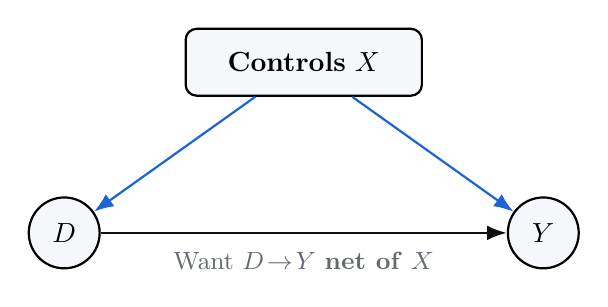
\begin{tikzpicture}[
      every node/.style={font=\normalsize},
      circ/.style={draw,circle,thick,fill=soft,
        minimum size=0.9cm}
    ]
      \node[draw,rounded corners,thick,fill=soft,
        minimum width=3cm,minimum height=0.85cm]
        (X) {\textbf{Controls\;}$X$};
      \node[circ,below left=1.4cm and 1.2cm of X]  (D) {$D$};
      \node[circ,below right=1.4cm and 1.2cm of X] (Y) {$Y$};

      \draw[-{Latex[length=2.5mm]},thick,accent] (X)--(D);
      \draw[-{Latex[length=2.5mm]},thick,accent] (X)--(Y);
      \draw[-{Latex[length=2.5mm]},thick,ink]    (D)--(Y);

      \node[below=0.12cm of $(D)!0.5!(Y)$,
        font=\small,text=muted]
        {Want $D\!\to\!Y$ \textbf{net of} $X$};
    \end{tikzpicture}
  \end{center}

  \swipe
\end{SafeFrame}

% ---- Prediction vs causation ----
\subsection{Prediction vs.\ Causation}

\begin{SafeFrame}{Where ML helps (and hurts)}
  \tagpill{Setup}\hspace{0.15cm}\tagpill{ML trade-off}

  \vspace{0.15cm}
  Model the world flexibly:
  \[Y = \beta\,D + g(X) + \varepsilon\]
  {\small\color{muted}%
    $g(X)$ = complex background effects.}

  \vspace{0.2cm}
  \begin{itemize}\setlength\itemsep{4pt}
    \item ML learns $g(X)$ well — great for prediction.
    \item But regularisation can \textbf{distort}~$\beta$.
  \end{itemize}

  \vspace{0.2cm}
  \callout{\textbf{Double ML idea:}
    let ML handle background chores,
    then estimate~$\beta$ on \emph{cleaned} data.}

  \swipe
\end{SafeFrame}

% ============================================================
\section{Double ML: Clean First, Estimate Second}
% ============================================================

\sectionbreak{Part 2}{Clean first, then estimate}

% ---- Workflow ----
\subsection{Workflow Pipeline}

\begin{SafeFrame}{Double ML workflow}
  \tagpill{Pipeline}\hspace{0.15cm}\tagpill{Steps}

  \vspace{0.15cm}
  \begin{center}
    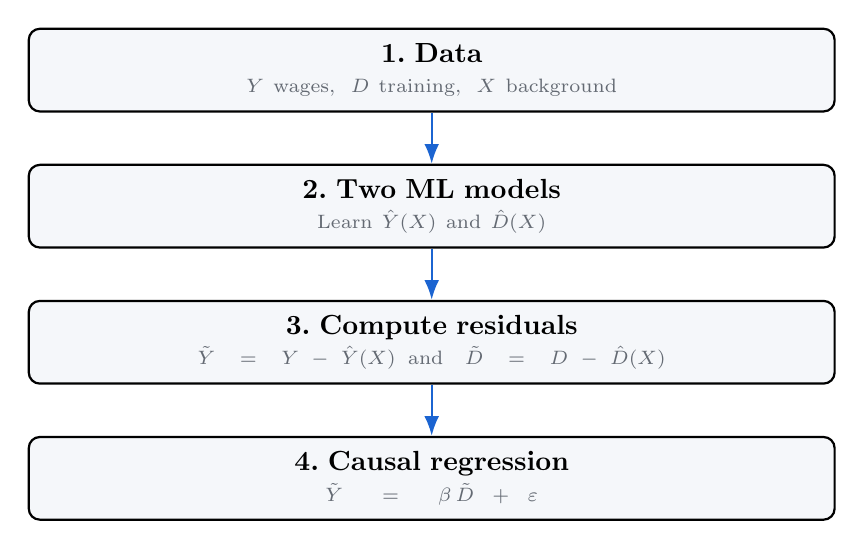
\begin{tikzpicture}[
      node distance=0.65cm,
      box/.style={draw,rounded corners,thick,fill=soft,
        text width=10cm,minimum height=1.05cm,
        align=center,font=\normalsize},
      arr/.style={-{Latex[length=2.5mm]},thick,accent}
    ]
      \node[box](s1){\textbf{1.\;Data}\\[-1pt]
        \scriptsize\color{muted}%
        $Y$ wages,\; $D$ training,\; $X$ background};
      \node[box,below=of s1](s2){\textbf{2.\;Two ML models}\\[-1pt]
        \scriptsize\color{muted}%
        Learn $\hat Y(X)$ and $\hat D(X)$};
      \node[box,below=of s2](s3){\textbf{3.\;Compute residuals}\\[-1pt]
        \scriptsize\color{muted}%
        $\tilde Y=Y-\hat Y(X)$\;\;and\;\;
        $\tilde D=D-\hat D(X)$};
      \node[box,below=of s3](s4){\textbf{4.\;Causal regression}\\[-1pt]
        \scriptsize\color{muted}%
        $\tilde Y=\beta\,\tilde D+\varepsilon$};

      \draw[arr](s1)--(s2);
      \draw[arr](s2)--(s3);
      \draw[arr](s3)--(s4);
    \end{tikzpicture}
  \end{center}

  \vspace{0.1cm}
  \callout{\textbf{Key:} estimate~$\beta$ from the part
    of training \emph{not explained by}~$X$.}

  \swipe
\end{SafeFrame}

% ---- Equations ----
\subsection{Orthogonalisation Equations}

\begin{SafeFrame}{The ``leftovers'' idea}
  \tagpill{Equations}\hspace{0.15cm}\tagpill{Meaning}

  \vspace{0.2cm}
  \begin{beamercolorbox}[rounded=true,wd=\linewidth,sep=8pt]{block body}
    \textbf{Step A\;— predict with controls:}
    \[\hat Y(X)\approx\mathbb{E}[Y|X],\qquad
      \hat D(X)\approx\mathbb{E}[D|X]\]

    \textbf{Step B\;— subtract predictions:}
    \[\tilde Y=Y-\hat Y(X),\qquad
      \tilde D=D-\hat D(X)\]
  \end{beamercolorbox}

  \vspace{0.25cm}
  \callout{\textbf{Causal step:}\;
    $\tilde Y=\beta\,\tilde D+\varepsilon$\\[3pt]
    The slope~$\beta$ \emph{is} the treatment effect.}

  \swipe
\end{SafeFrame}

% ============================================================
\section{Data Example}
% ============================================================

\sectionbreak{Part 3}{Data example (wage / labour)}

\subsection{Toy Dataset}

\begin{SafeFrame}{Illustrative dataset}
  \tagpill{Data}\hspace{0.15cm}\tagpill{Readable}

  \vspace{0.15cm}
  \begin{beamercolorbox}[rounded=true,wd=\linewidth,sep=6pt]{block body}
    $Y$: wage (\$/mo)\quad
    $D$: training (0/1)\quad
    $X$: educ \& exp
  \end{beamercolorbox}

  \vspace{0.25cm}
  \begin{center}
    \begin{tabular}{@{}lcccc@{}}
      \toprule
      Person & $D$ & Educ & Exp & Wage\\
      \midrule
      A & 1 & 16 & 6 & \$3\,900\\
      B & 1 & 14 & 5 & \$3\,400\\
      C & 1 & 12 & 4 & \$2\,950\\
      D & 0 & 16 & 6 & \$3\,650\\
      E & 0 & 14 & 5 & \$3\,150\\
      F & 0 & 12 & 4 & \$2\,700\\
      \bottomrule
    \end{tabular}
  \end{center}

  \vspace{0.15cm}
  \callout{\textbf{In practice:} $X$ can have hundreds
    of variables. Double ML scales the same way.}

  \swipe
\end{SafeFrame}

% ============================================================
\section{Visual Evidence}
% ============================================================

% ---- Wage vs Education ----
\subsection{Wages vs.\ Education}

\begin{SafeFrame}{Wages rise with education}
  \tagpill{Plot}\hspace{0.15cm}\tagpill{Confounding}

  \vspace{0.1cm}
  \begin{itemize}\setlength\itemsep{2pt}
    \item Education predicts wages strongly.
    \item If trainees are more educated,
          the raw gap overstates the effect.
  \end{itemize}

  \vspace{0.15cm}
  \begin{center}
    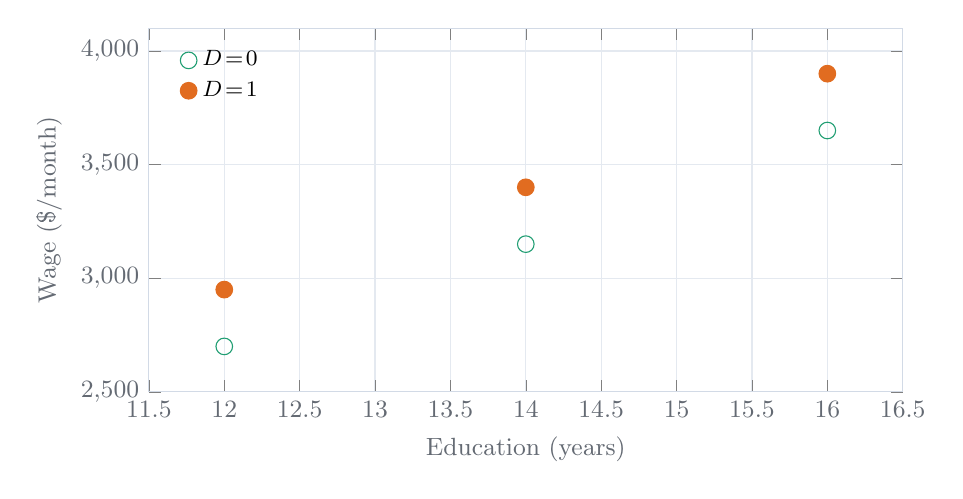
\begin{tikzpicture}
      \begin{axis}[
        width=0.92\linewidth,
        height=6.2cm,
        xlabel={Education (years)},
        ylabel={Wage (\$/month)},
        ticklabel style={font=\small,color=muted},
        label style={font=\small,color=muted},
        axis line style={draw=linegray},
        grid=major,
        grid style={draw=linegray!60},
        xmin=11.5,xmax=16.5,
        ymin=2500,ymax=4100,
        legend style={font=\footnotesize,draw=none,fill=none,
          at={(0.03,0.97)},anchor=north west}
      ]
        \addplot[only marks,mark=o,mark size=3pt,accentgreen]
          coordinates{(12,2700)(14,3150)(16,3650)};
        \addlegendentry{$D\!=\!0$}
        \addplot[only marks,mark=*,mark size=3pt,accentorange]
          coordinates{(12,2950)(14,3400)(16,3900)};
        \addlegendentry{$D\!=\!1$}
      \end{axis}
    \end{tikzpicture}
  \end{center}

  \vspace{0.08cm}
  \callout{\textbf{Double ML:} remove the education /
    experience part \emph{first}.}

  \swipe
\end{SafeFrame}

% ---- Residual plot ----
\subsection{Residual Plot}

\begin{SafeFrame}{Effect in the leftovers}
  \tagpill{Residuals}\hspace{0.15cm}\tagpill{Causal step}

  \vspace{0.1cm}
  After cleaning out~$X$, the slope reveals
  the causal effect:

  \vspace{0.15cm}
  \begin{center}
    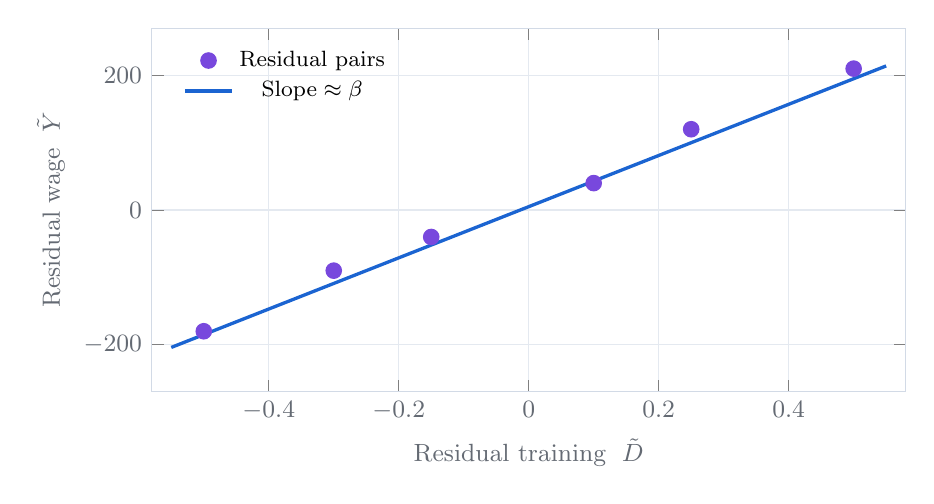
\begin{tikzpicture}
      \begin{axis}[
        width=0.92\linewidth,
        height=6.2cm,
        xlabel={Residual training\; $\tilde D$},
        ylabel={Residual wage\; $\tilde Y$},
        ticklabel style={font=\small,color=muted},
        label style={font=\small,color=muted},
        axis line style={draw=linegray},
        grid=major,
        grid style={draw=linegray!60},
        xmin=-0.58,xmax=0.58,
        ymin=-270,ymax=270,
        legend style={font=\footnotesize,draw=none,fill=none,
          at={(0.03,0.97)},anchor=north west}
      ]
        \addplot[only marks,mark=*,mark size=2.8pt,accentpurple]
          coordinates{
            (-0.50,-180)(-0.30,-90)(-0.15,-40)
            (0.10,40)(0.25,120)(0.50,210)};
        \addlegendentry{Residual pairs}
        \addplot[domain=-0.55:0.55,samples=2,
          very thick,accent]{380*x+5};
        \addlegendentry{Slope\;$\approx\beta$}
      \end{axis}
    \end{tikzpicture}
  \end{center}

  \vspace{0.08cm}
  \callout{$\tilde Y=\beta\,\tilde D+\varepsilon$
    \;— the slope \emph{is} the causal effect.}

  \swipe
\end{SafeFrame}

% ============================================================
\section{Takeaway}
% ============================================================

\begin{SafeFrame}{Final takeaway}
  \tagpill{Summary}

  \vspace{0.4cm}
  \callout{%
    \textbf{Double ML} uses machine learning to
    strip out background effects~($X$), then
    estimates the causal effect from leftover
    variation only.}

  \vspace{0.35cm}
  \begin{beamercolorbox}[rounded=true,wd=\linewidth,sep=10pt]{block body}
    {\Large\textbf{Clean first, then estimate.}}\\[5pt]
    \color{muted}\normalsize
    Orthogonalisation makes the causal estimate
    robust to ML prediction errors in the
    nuisance parts.
  \end{beamercolorbox}

  \vfill
  \hfill{\color{muted}\small End}
\end{SafeFrame}

% ============================================================
%  THANK YOU
% ============================================================
\section*{}

\pdfbookmark[0]{Thank You}{thankyou}
\begin{frame}[plain]
  \vfill
  \begin{center}
    {\fontsize{26}{30}\selectfont\bfseries\color{ink}%
      Thank You}\\[0.8cm]
    {\Large Muiz Olasupo}\\[0.3cm]
    {\normalsize\color{muted}Causal Inference in Economics}
  \end{center}
  \vfill
\end{frame}

\end{document}